\section{Results}

To test the accuracy of our model, we perform Leave One Out (LOO) Cross Validation. This form of cross validation involves using one observation as the validation set and the remaining observations as the training set. This is repeated for all combinations of training sets, allowing every observation to act as a validation set. For our analysis an observation is one set of configurations. For example, consider five sets of configurations: A through E. We pick A as the validation set and train the model on all other configurations.\\

For a single test, our program will now "walk through" rebuilding configuration A token-by-token, starting from the first keyword. At every step, we invoke our model and compare our predictions against the actual tokens in A. If the model generates the correct prediction within the top three results, we mark a token completion to be successful. We tally up the number of model invocations and the number of correct predictions.\\
 
\begin{figure}[H]
	\centering
	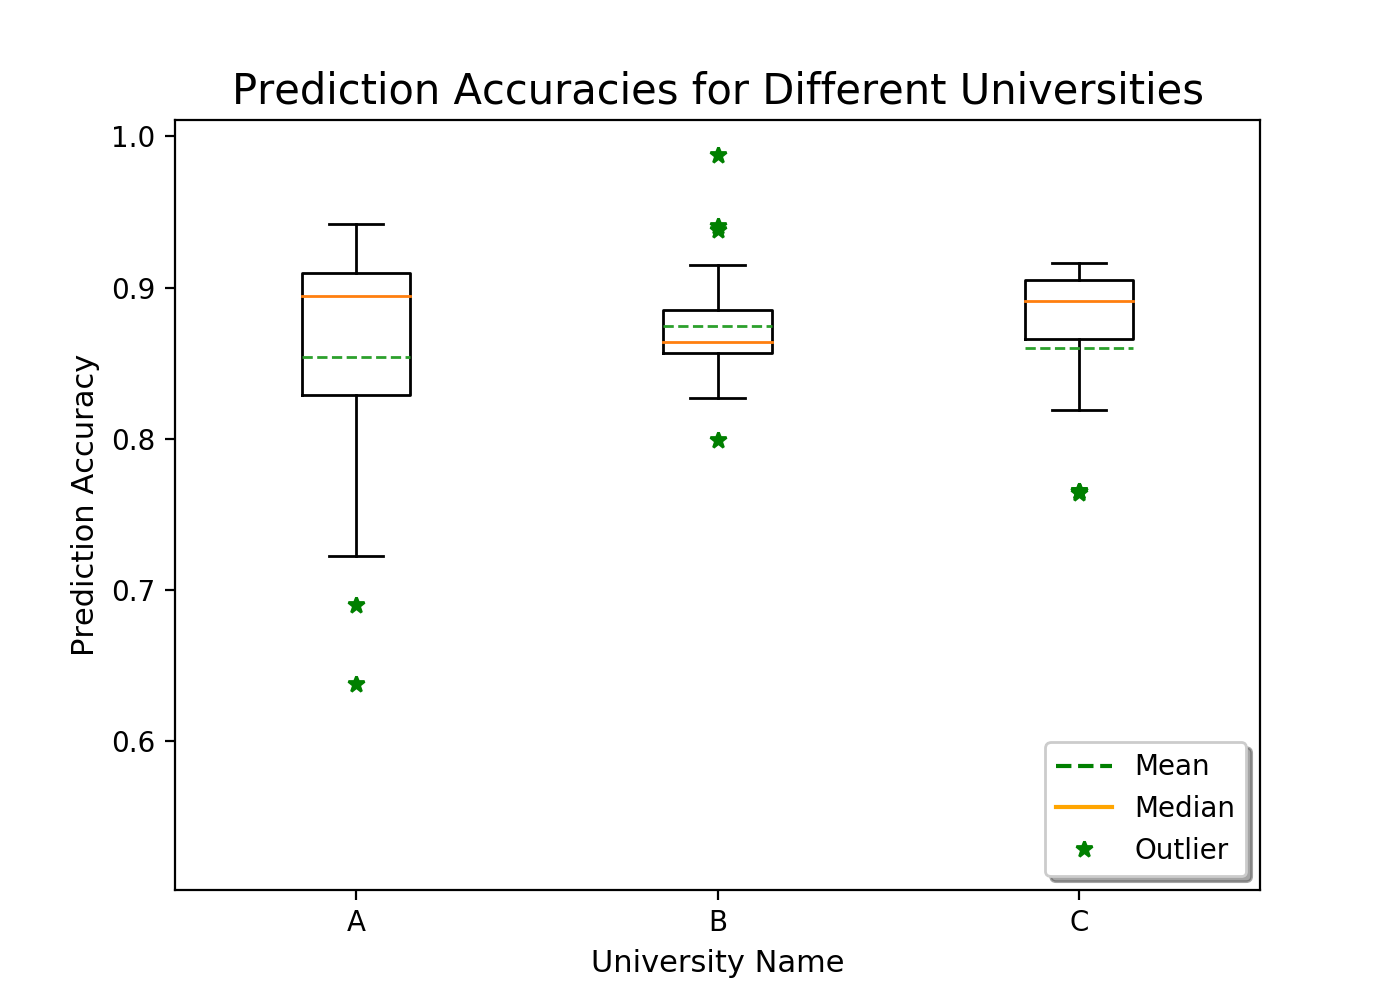
\includegraphics[width=5in]{uni_analysis.png}
	\caption{Overall accuracy of the model for each set of university configurations used as the validation set.}
\end{figure}

In the figure shown above, the the x-axis shows the name of the three anonamyzed universities used, and prediction accuracies on the y-axis. The box plot is supposed to highlight the average (green dotted line), median (orange line) and upper ($Q_U$) and lower quartiles ($Q_L$). The box itself marks the Inter Quartile Range (IQR). The outliers (green stars) are all the data points that lie outside $Q_L - 1.5*IQR$ and $Q_U+1.5*IQR$.\\

Initially, without any preprocessing and subnet removal, we observed a maximum accuracy of 85\% and an average of 65\%. Our results in the figure above are after preprocessing the data and we now see accuracies as high as 93\%, and an average of 81\%. These results are very promising as we see a significant jump in accuracy from simple refinements to the model. More placeholders would improve accuracies even further but with diminishing returns.


\subsection{Evaluations}

There were a myriad of analyses we performed in order to test the efficacy of an ngram-based engine as described in the previous section. In this section we discuss some which produced interesting results. We first describe the general trend we observed when we implemented placeholder. Next, we outline how our analyses show that across both dimensions of time and length, the NLP algorithm is resistant to data scarcity. Furthermore, we showed how breaking up the configurations by router roles gave us unexpected results.

\subsubsection{Placeholders}

\begin{figure}[H]
	\centering
	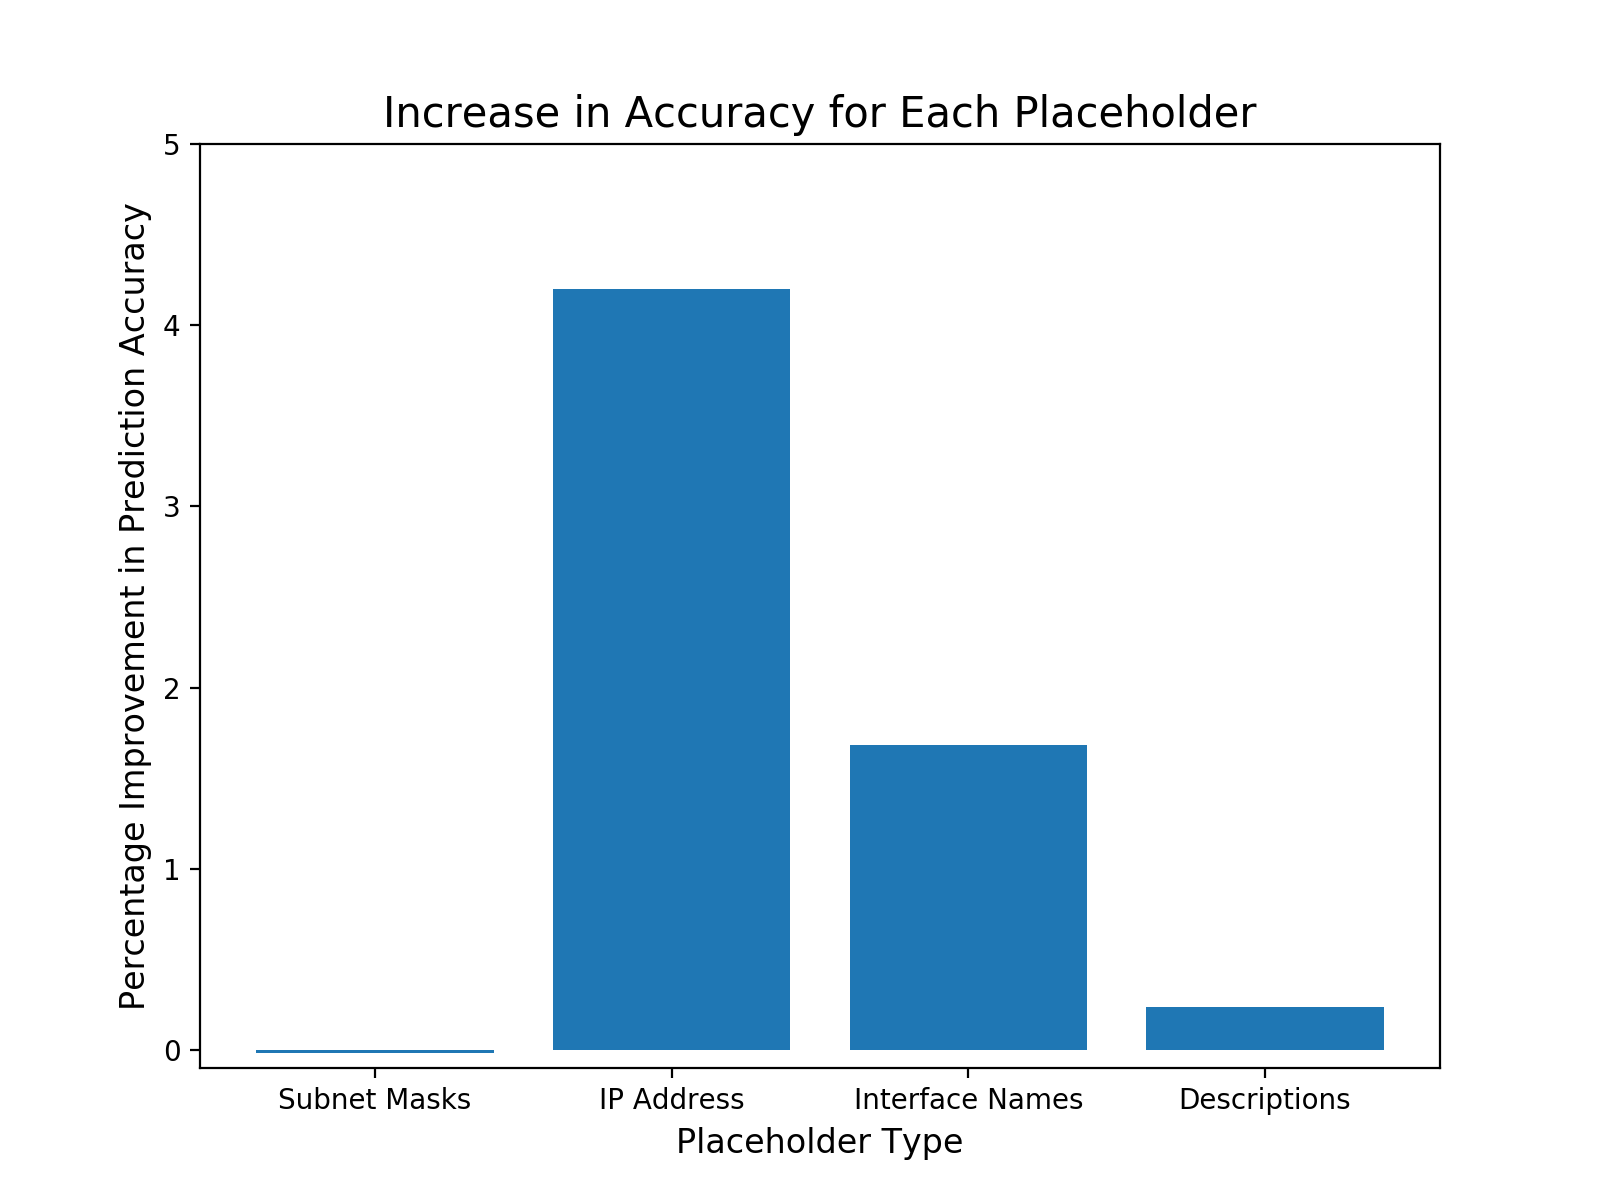
\includegraphics[width=\textwidth]{placeholders.png}
	\caption{Effect on Accuracy by Every Placeholder}
\end{figure}

Generally, we see an improvement when placeholders are used to substitute certain keywords. As the graph shows, the biggest jump in accuracy is accomplished by using IP address placeholders. This is expected, as configurations are bound to consist of a number of unique IP addresses which it makes it extremely difficult to predict which one is going to be used. Other tokens, for example subnet masks, tend to be much more homogeneous (usually a handful of subnet masks are repeatedly used across a network). As placeholders were resulting in diminishing returns, due to time constraints, we decided to go ahead with the ones we had implemented. We leave additional placeholders as a possible future extension.


\subsubsection{Length of Histories}

\begin{figure}[H]
	\centering
	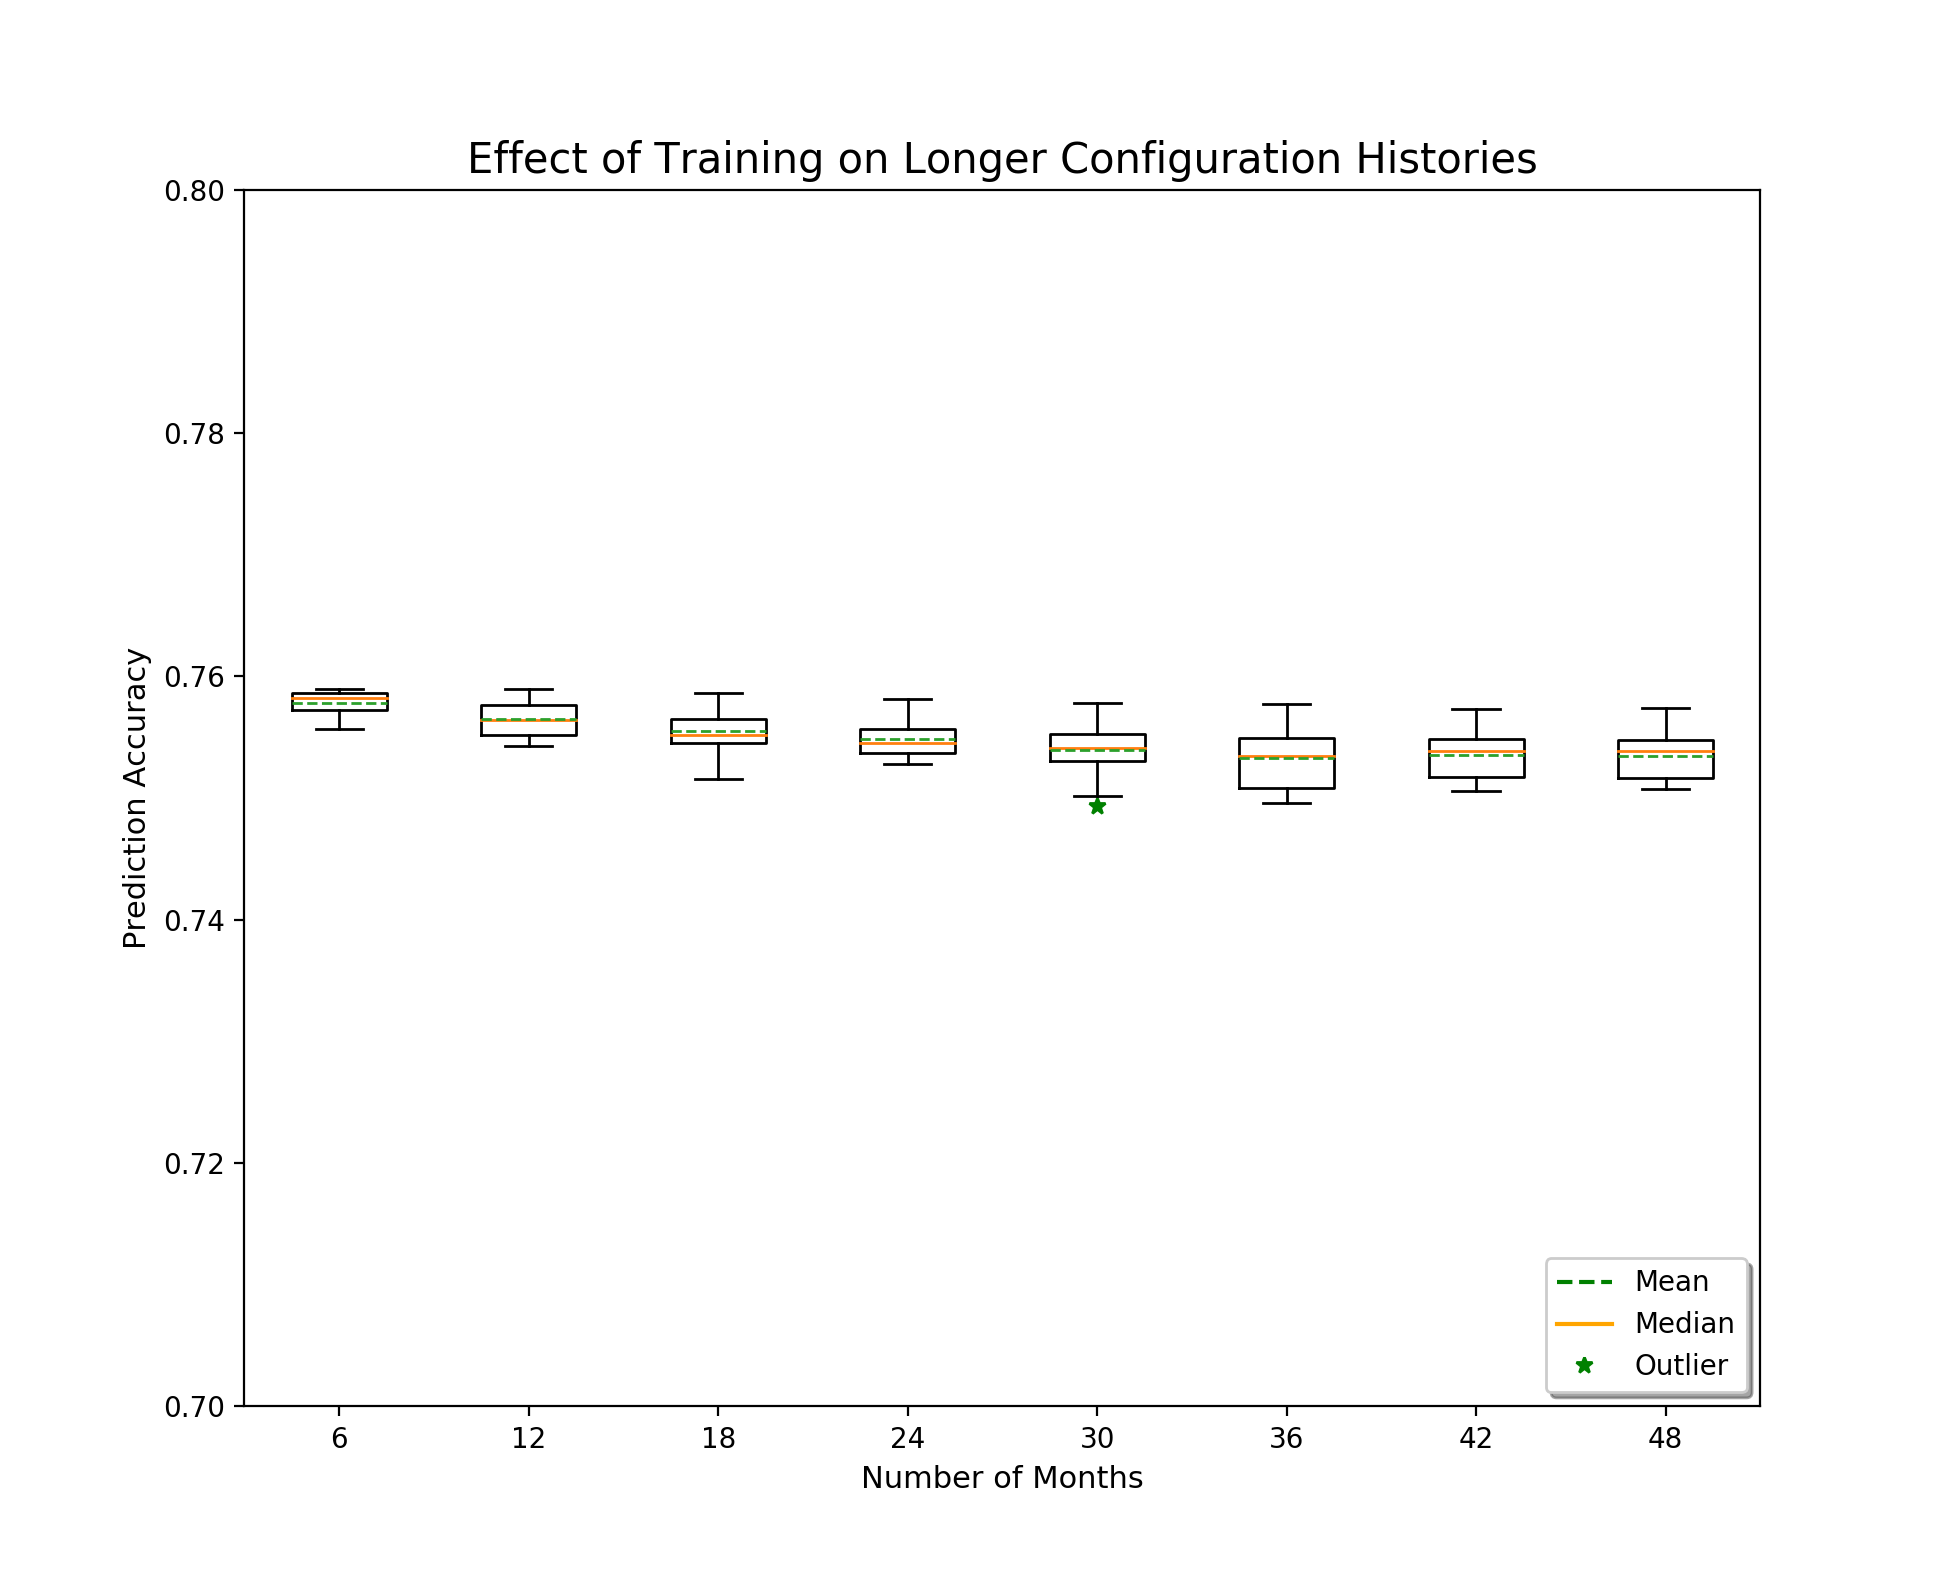
\includegraphics[width=\textwidth]{time.png}
	\caption{Longer histories may not result in higher accuracies.}
\end{figure}

As we had extensive data from University A's version control system, we analyzed the effect of selecting configurations across time on prediction accuracies. The x-axis of the graph shows the number of months we chose to train on. As is apparent from the image, if we train on longer configuration histories our accuracies stay about the same. In fact, we see a slight decrease which may be attributed to the variation introduced by the increased data points. We do expect some change in the configurations over time as the university networks evolve. However, these changes tend to be small and homogeneous as the analyses from from ~\cite{Kim} inform us. Thus, our model does not need to consider configurations across 4 years for this university.

\subsubsection{Number of Devices}
\begin{figure}[H]
	\centering
	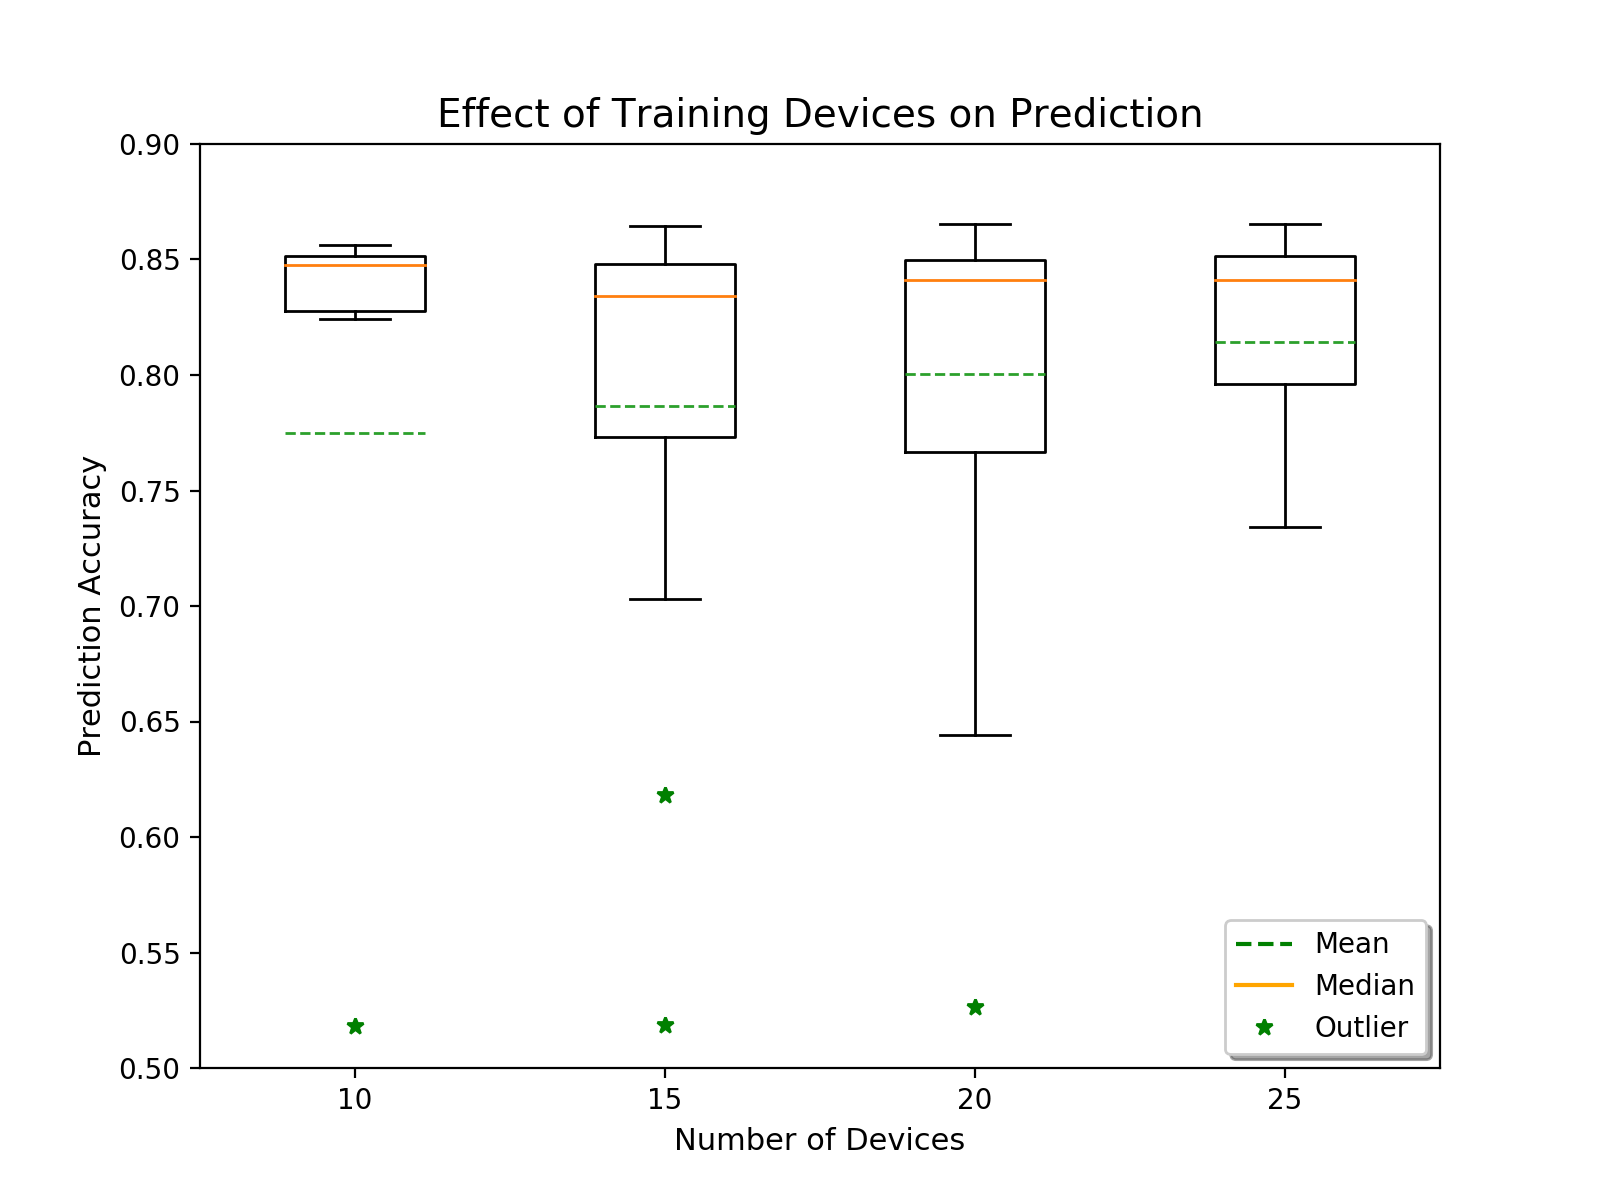
\includegraphics[width=\textwidth]{device_analysis.png}
	\caption{Training across more devices does improve accuracy to a certain point.}
\end{figure}

As we add configurations from more devices to our training set, we see a slight increase in accuracy before it starts to give us diminishing returns. This may mean that the model has already seen most of the tokens that are often used by network operators. Every additional device contributes less to the overall model prediction set. In practice some devices being added may be different from the rest of the network, causing them to act as outliers which would be affecting our averages.

\subsubsection{Role-Based}

\begin{figure}[H]
	\centering
	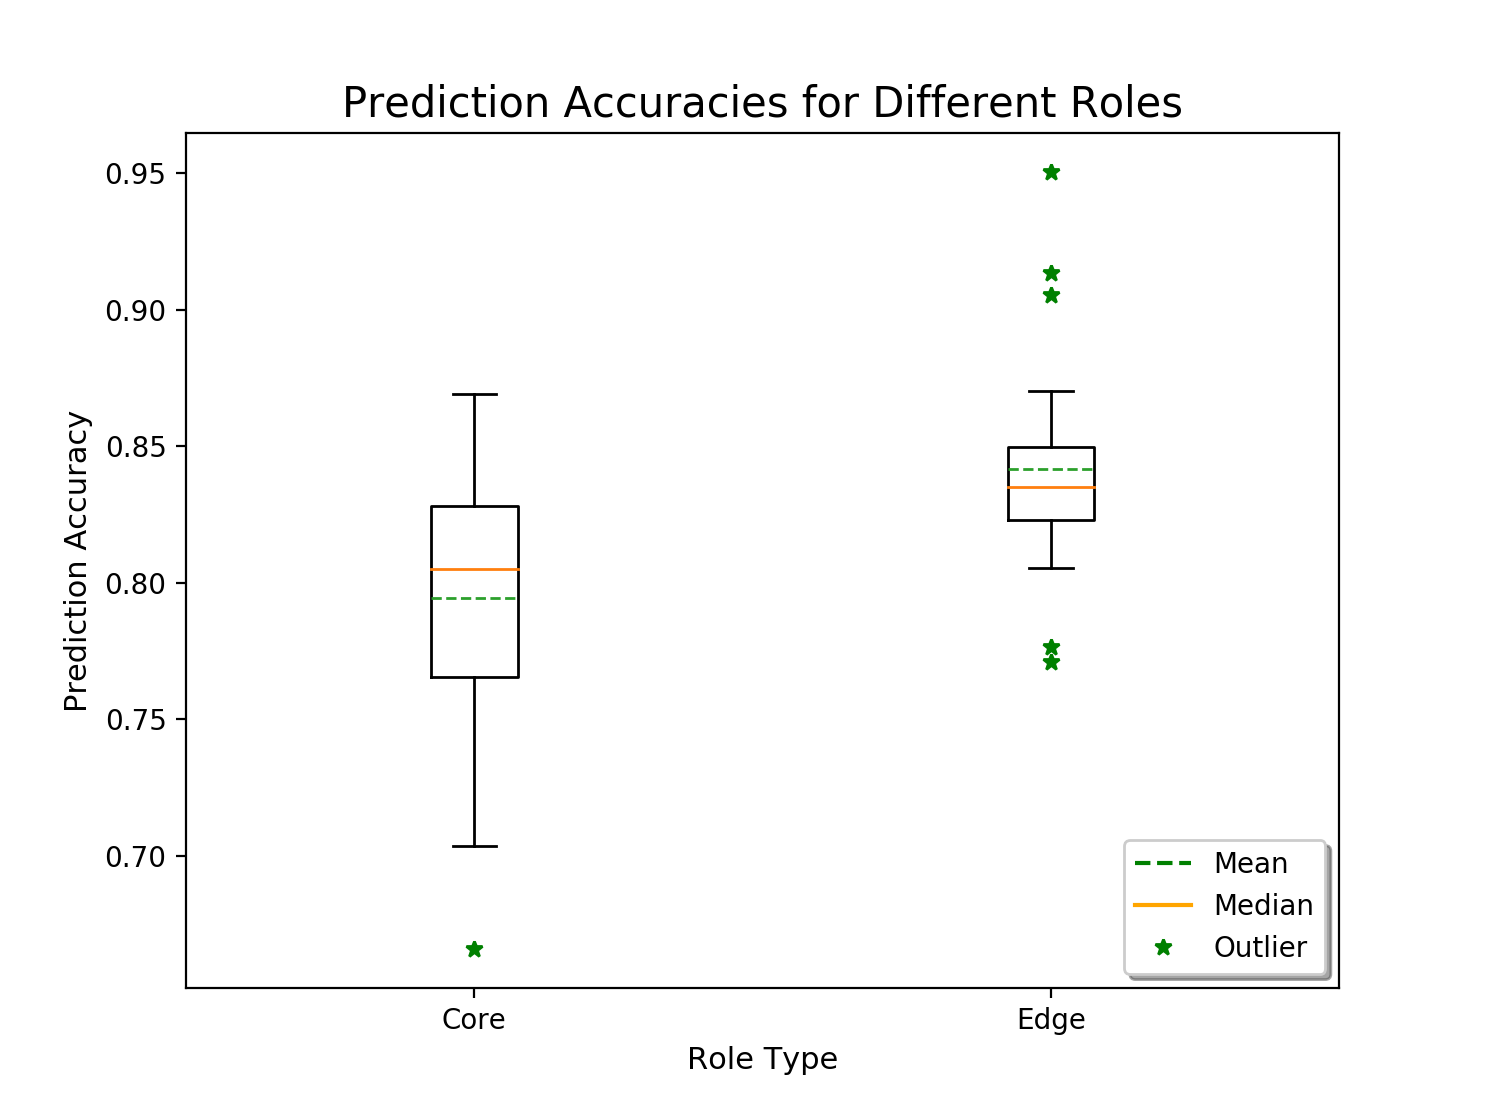
\includegraphics[width=\textwidth]{roles.png}
	\caption{Accuracies of models were trained on core and edge routers only, with the first boxplot showing the combined training set}
\end{figure}

Splitting by roles did not result in an improvement in accuracy like we expected. There are a few factors that could be contributing to this result. It might be possible that there is not much variation in the two roles to begin with. We were assuming that the suggestions generated by the "combined" version would contain the tokens for both edge routers and core routers which would reduce the chances of the correct one cropping up in the top 3 suggested tokens. However, the results show that after separation, edge routers did not fare any better and core routers actually did worse. We also believe that this may be a problem of the labels/roles being coarsely defined as we were relying on the names of the routers to separate them. It is entirely possible that network operators may be labeling the routers as a rough approximation of their intended roles. Thus researchers may need to figure out a more fine grained way about dividing them.

